\documentclass[12pt, letterpaper]{article}
% \documentclass[12pt, notitlepage]{report}

%% Language and font encodings
\usepackage[english]{babel}
\usepackage[utf8x]{inputenc}
\usepackage[T1]{fontenc}

%% Sets page size and margins
\usepackage[letterpaper,top=2.54cm,bottom=2.54cm,left=2.54cm,right=2.54cm]{geometry}
% ,marginparwidth=1.75cm
\usepackage{multicol}
% \usepackage{parskip}
\usepackage{natbib}

%% Useful packages
\usepackage{amsmath}
\usepackage{graphicx}
\usepackage[colorinlistoftodos]{todonotes}
\usepackage[colorlinks=true, allcolors=blue]{hyperref}
\usepackage{float}
\usepackage{booktabs}
\usepackage{array}

\usepackage{abstract}
\setlength{\absleftindent}{0mm}
\setlength{\absrightindent}{0mm}
\renewcommand{\abstractnamefont}{\normalsize\bfseries}

\usepackage{sectsty}
\sectionfont{\fontsize{12}{12}\selectfont}

\title{\vspace{-6ex}Understanding Code-Mixed Dialogues in Context\vspace{-4ex}}

\date{}

\begin{document}
\maketitle
\begin{multicols*}{2}
% \setlength{\parskip}{0.1in}
\setlength{\parindent}{15pt}

\begin{abstract}
\normalsize
Code-mixing occurs when people use multiple languages to communicate. In order to understand code-mixing in context, we develop a bilingual goal-oriented dialogue system that will try to talk to human users in various styles of Spanish-English code-mixing. Our system involves modifying an existing monolingual dialogue framework to transform the English output into 3 different styles of Spanish-English code-mixing: syntactic, lexical, and social. In this ongoing exploratory work, we have the pipeline built and will soon be releasing this system on Amazon Mechanical Turk to gather conversations of our system with crowdsourced bilinguals. From these dialogues, we will then measure the levels of entrainment of these 3 styles from the users’ text responses.
\end{abstract}

\normalsize
\section{Introduction} 
The prevalence of code-mixing has been increasing with globalization and the rise of multilinguality, as found in speech and on social media. Existing human language technologies lack the ability to adequately handle processing utterances of multiple languages, and they need to accommodate people who code-mix. From both fields of Linguistics and Natural Language Processing have emerged studies on areas such as predicting switch-points within utterances, or enhancing language modeling for code-mixed speech recognition \citep{Solorio2008,Li2014}. However, we want to understand code-mixing in a wider context of a dialogue between two people, and effectively learn about the bilingual mind and the linguistic and social triggers of code-mixing.

Entrainment in dialogue has been well-studied as a basis of human interaction and rapport, with past work dealing in areas of lexical choice, syntax, acoustics, etc. \citep{Levitan2013}. It is essentially when dialogue partners adapt speech styles to each other over time. Even though we want to use entrainment as the means by which to understand code-mixing, the field of entrainment itself can benefit from our work, because code-mixing is an additional dimension of rapport that has not yet been studied.

Perhaps the most closely related work to our proposed chatbot is a human-machine dialogue system from \citet{Ramanarayanan2017}, who produced a set of Spanish-English and Hindi-English machine prompts to encourage human bilinguals to code-mix back to the machine. 

Since we wanted to implement an existing task-oriented system to ground the dialogue while still remaining flexible in the topics of discussion, we use the scenario of discussing mutual friends given a knowledge base, previously done by \citet{he2017learning}. According to this framework called CoCoA, both users of a system (in our case, one human and one machine) will have a private table of “friends” with certain attributes such as their hobbies and location preferences. Only one friend will be the same across the two users’ tables, so the goal is to collaboratively discuss and select that mutual friend. In our version, we update the knowledge bases and system output to be bilingual.

\section{Methodology}
We use CoCoA's rule-based monolingual text English generation as the basis for our three main bilingual style transformations, namely: (1) syntactic, (2) lexical, and (3) social. Syntactic style involves mixing at higher phrase-level boundaries--potentially a more periodic way of switching languages. Lexical style has a set of content words in one language while the function words remain in the other. Social style includes things like changing level of formality and expressing opinions versus fact. Examples of each of these are shown below:

\vspace{2ex}
\noindent
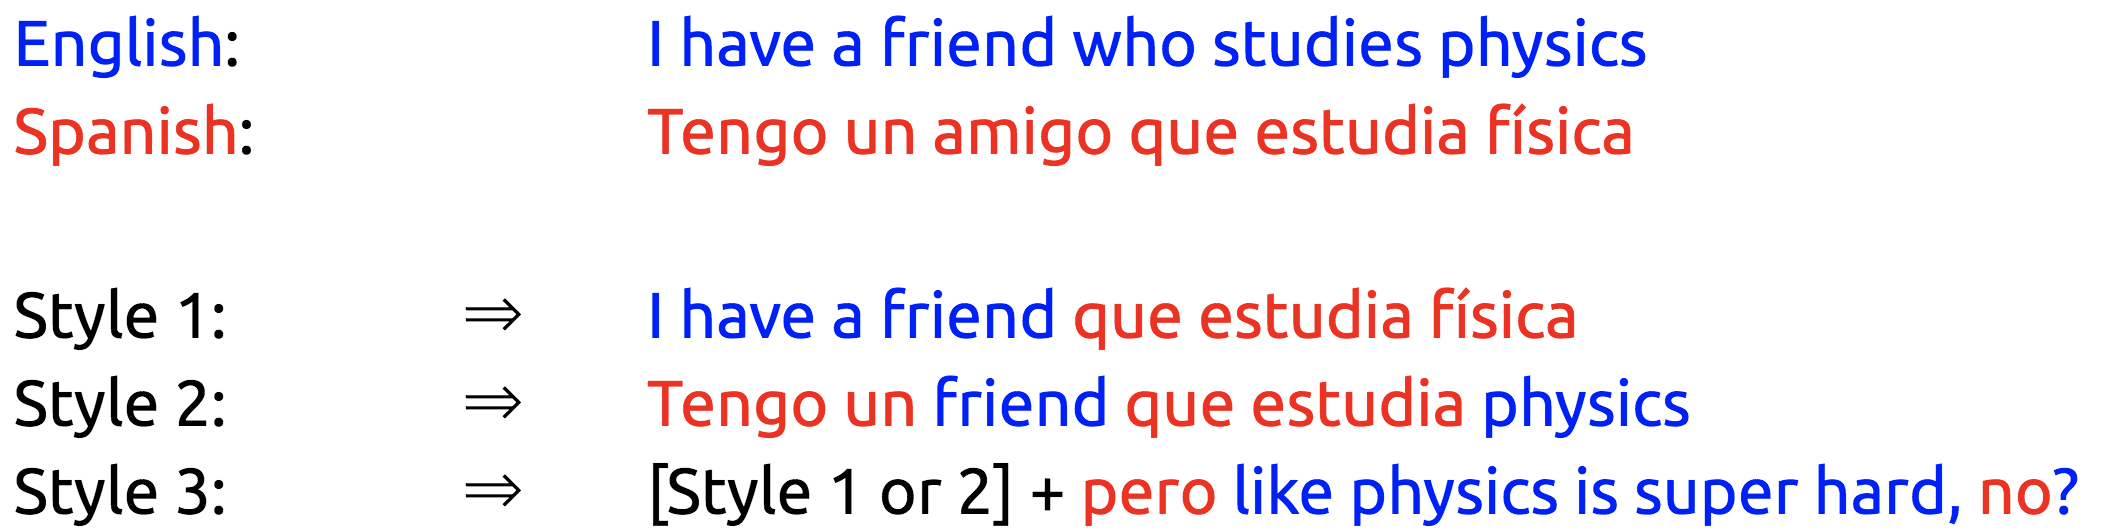
\includegraphics[width=8.2cm]{style_ex}
% \vspace{1ex}

Following the architecture shown in the figure below, we add the relevant portions (in green) to the existing monolingual generation of CoCoA’s rule-based chatbot (in blue). Not pictured is the way for the user output to be transferred back to CoCoA via basic entity-linking, after being normalized into monolingual English.

% \vspace{2ex}
\noindent
% 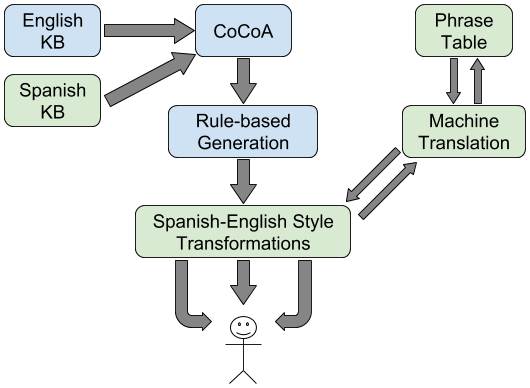
\includegraphics[width=8.2cm]{bl_cocoa}
\begin{center}
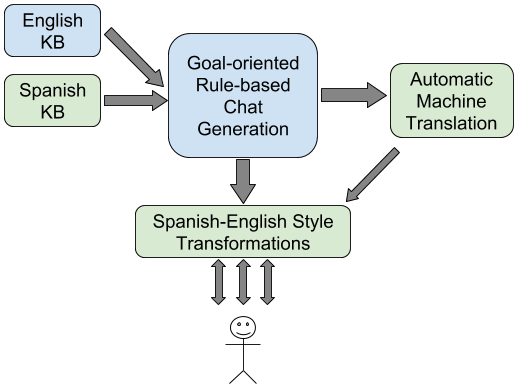
\includegraphics[width=7cm]{fig1_0307}
\end{center}

% \vspace{1ex}

\section{Experimental Setup}

As part of our current ongoing work, we will release the full dialogue system first as a pilot study with few known bilinguals, and then in batches of 20 crowdsourced bilinguals on Amazon Mechanical Turk. After doing text normalization and language identification on the responses, we will calculate entrainment scores for things such as the amount of code-mixing and the presence of certain content words indicating each of our styles.

\section{Conclusion}
Entraining the user to our styles will allow us to examine the nature of code-mixing in a controlled way. This exploratory work will specifically try to answer the question: How will Spanish-English bilinguals respond to a chatbot that produces different styles of code-mixing? But in a broader sense, language technologies can learn from code-mixing in dialogues, and personalization of AI systems can hopefully entrain back to users, which would lead to more natural interactions for humans and machines. Future work can also be done on other language pairs such as Hindi-English, leading to analysis on how linguistically and functionally similar or different the style entrainment would be, compared to Spanish-English.

\bibliography{nasslli}
\bibliographystyle{acl_natbib}

\end{multicols*}
\end{document}
